\section{Preliminaries} \label{sec:preliminaries}
In this section we give a more detailed overview of the properties of the NDN architecture relevant to the issue of anonymous communication. We then also delve into the design of AND\=aNA (henceforth referred to as AND\=aNA-v1), to identify the major security flaws and engineering shortcomings that are remedied in AND\=aNA-v2. 

\subsection{NDN Overview}
Named-data networking (NDN) is one of several proposed information-centric network designs under active research and development as the future Internet architecture. Its defining characteristic is that it decouples the location of data from its original publisher. All requested content is cached in network-layer routers between consumers who request data and publishers, or other routers, satisfying such data. In essence, network caches and addressable content, rather than addressable hosts or interfaces, enable this new architecture to reduce network congestion and latency by keeping content closer to its intended recipients. 

Content is requested through the issuance of an \emph{interest}, or a meaningful URI with a one-to-one correspondence with content provided by the network. The components of an interest are arbitrary strings and can therefore be used to store any type of data, including human readable names or binary data encoded as URI-friendly strings. Upon receiving an interest, a router looks for a match in its \emph{content store} (CS), which is the cache that stores content already requested from other consumers. Matching is done using exact-match based on content names, i.e., a complete interest name match in the CS will cause the associated content to be forwarded downstream on the same router interface upon which the interest arrived. Interests that do not completely match any content name in the CS are stored in a \emph{pending interest table} (PIT) together with the corresponding interface upon which the interest arrived and is subsequently forwarded to the appropriate upstream router based on contents in a \emph{forward interest base} (FIB) table. Multiple interests matching the same name are collapsed into a single PIT entry to prevent redundant interests being sent upstream. Once a content matching a PIT entry is received by a router, the content is cached (unless the interest has explicitly marked the content to not be stored) and sent to all downstream interfaces associated with the PIT entry. Finally, upon completion, the PIT entry is cleared.

Content-centric traffic also has strong security implications. Firstly, it means that content security is tied to the data itself, not the channel through which it flows between consumers and the network. All sensitive content must therefore be protected with a suitable form of encryption to ensure confidentiality. Content integrity is guaranteed by digital signatures; all content producers are required to sign content before responding to incoming interests. Due to performance impediments, signature verification is not required by network routers; naturally, consumer applications are expected to verify content signatures. Issues regarding signature verification and key management are discussed more at length in \cite{}.Secondly, a lack of source and destination addresses improves user privacy. However, as we will discuss in the following section, this lack of information is insufficient with regards to consumer privacy. 

\subsection{Notions of Anonymity}
\todo[inline]{I think a section dedicated to anonymity and relevant definitions is warranted here, oui?}

\subsection{AND\=aNA-v1 Design Highlights}
Section \ref{sec:design} provides a detailed description of the design of {\sf AND\=aNA-v2}, which is inspired by Tor and its predecessor, {\sf AND\=aNA-v1}. To motivate our changes we first describe the {\sf AND\=aNA-v1} design in sufficient detail. As previously mentioned, {\sf AND\=aNA-v1} achieves anonymous communication using mix behavior analogous to Tor; Interests for content are wrapped in layers of encryption, where each encrypted layer has sufficient information necessary to forward the interest to the correct anonymizing router. Note that unlike Tor, persistent circuits with long-term TCP connections are not established with {\sf AND\=aNA-v1}. Rather, ephemeral circuits are created as an interest is decrypted and forwarded upstream towards the consumer. State information in each anonymizing router is only maintained in the symmetric (session-based) variant of {\sf AND\=aNA-v1}. Once a piece of content is retrieved corresponding to an interest, each anonymizing router wraps it with a layer of encrypting using a public or symmetric key specific in the corresponding interest, and is subsequently sent back downstream. In this way, circuits only exist for the duration of a single interest-content retrieval. This behavior is illustrated in Figure \ref{fig:andanav1_design}.

\begin{figure}
\begin{center}
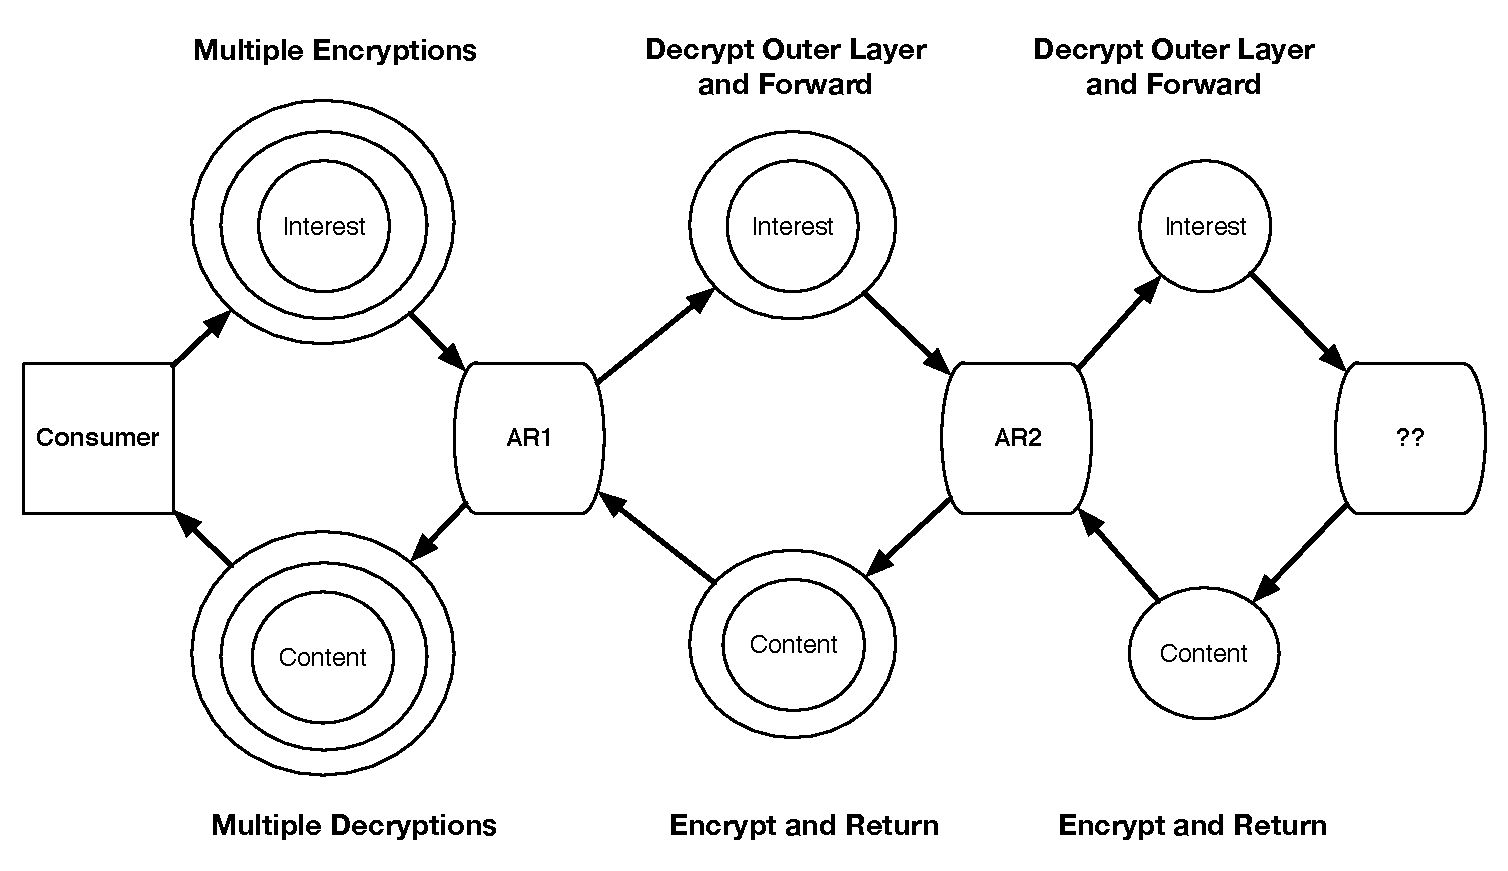
\includegraphics[scale=0.34]{./images/andana_v1_design.pdf}
\label{fig:andanav1_design}
\caption{Interest and content onion encryption and decryption in the original {\sf AND\=aNA-v1} design.}
\end{center}
\end{figure}

In the symmetric variant of {\sf AND\=aNA-v1}, state information consisting of a unique session identifier and symmetric key used for interest and content decryption and encryption, respectively, is established and persisted in each anonymizing router using a standard three-way handshake protocol. While the use of symmetric encryption removes the computational burden of asymmetric content encryption, the reference design required that the session identifier be sent in the clear for every interest, allowing an adversary to link packets and content together and render the consumer susceptible to a deanonymization attack (see the following section for more details). Furthermore, not only is the initial state establishment protocol composed of interests that are distinct from regular encrypted interests, the handshake procedure wastes consumer bandwidth and time when used for short-term anonymous traffic. 

\todo[inline]{We can probably go farther here - has the point been driven home?}

\subsection{Pitfalls and Shortcomings}
The primary motivation for a new design of {\sf AND\=aNA} is to attain the same anonymity and privacy guarantees as {\sf AND\=aNA} with \emph{better} performance. The original design targeted a single use case in which performance, especially in the bidirectional setting, was not a primary concern. Indeed, there was both an asymmetric and symmetric (session-based) variant of {\sf AND\=aNA}, and while the latter enjoyed better speedups over the former by using symmetric encryption it suffered the fatal flaw of not ensuring packet unlinkability. It is generally the case that unlinkability is merely sufficient for anonymity, rather than also being a necessary condition for anonymity. However, in the case of {\sf AND\=aNA}, packet linkability can lead to consumer and producer linkability, which immediately violates anonymity. For example, it is not difficult to hypothesize an adversary that eavesdrops on incoming and outgoing interests for a particular anonymous router, and who by doing so is able to determine that the incoming and outgoing session IDs are linked. In fact, a modified type of this kind of adversary was explicitly studied in the context of Tor by Murdoch and Danezis in \cite{tor-traffic-analysis}. In their work, the goal of the adversary in their ``linkability attack'' was to determine whether two separate data streams being served by two corrupted servers were initiated by the same consumer, and we suspect that such analysis could be augmented to work for {\sf AND\=aNA}. Specifically, repeating a packet linkability attack at each anonymous router in a circuit may therefore eventually lead to linkability between the producer and consumer. 

The use of application and environment contextual information has also been formally studied in \cite{attacking-unlinkability}, in which side channel and environment information (e.g., the deterministic behavior of an anonymous router always forwarding a packet upstead after unwrapping an interest received from some downstream router) is used to quantify the \emph{degree of unlinkability}. Furthermore, we remark that regardless of how such linkability information is acquired, it has been shown that it can lead to reduce consumer and producer anonymity beyond what is possible with general traffic analysis \cite{linkability-attacks}. 

As most of the literature focuses on mix-based anonymizing services akin to Tor, which inspired the original design of {\sf AND\=aNA}, it is clear that any form of linkability should be avoided in order to maintain consumer and producer anonymity. Therefore, one formal goal for {\sf AND\=aNA-v2} is to attain the same anonymity and privacy guarantees as the asymmetric variant of {\sf AND\=aNA}, which does not suffer from packet linkability issues, while supporting \emph{superior} performance in the low-latency, high-throughput, bidirectional traffic use case when compared to the symmetric variant of {\sf AND\=aNA}.
